\section{Data}\label{sec:data}
\subsection{Data Sources and Collection}
The empirical analysis leverages a curated macroeconomic panel constructed from publicly available and internally aggregated sources. Core indicators include real GDP (GDPC1), unemployment rate (UNRATE), consumer price index (CPIAUCSL), business dynamics statistics (BDS), and policy variables associated with \VAT{} adjustments. Datasets were sourced from recognized repositories (e.g., Federal Reserve Economic Data) and harmonized to a unified temporal frequency.

\subsection{Preprocessing and Harmonization}
Raw series were merged on a standardized date index, handling frequency mismatches via temporal aggregation or interpolation subject to preserving structural turning points. Missing observations were imputed using seasonally-aware methods where necessary, and outliers were screened through median absolute deviation thresholds. All nominal variables were deflated using the consumer price index base period normalization.

\subsection{Feature Engineering}
Derived covariates include lag structures (1--12 periods), rolling volatility, growth differentials, detrended components (HP-filter residuals), and interaction terms capturing joint labor-market and price dynamics. A policy event indicator flags periods surrounding implemented or proposed \VAT{} adjustments, enabling localized treatment effect estimation.

\subsection{Analytical Sample}
Observations with incomplete covariate histories within the lag window were excluded from model training to avoid leakage. The final analytical dataset balances temporal depth and multivariate richness, supporting both sequence learning and heterogeneous effect modeling.

\subsection{Descriptive Statistics}
Table~\ref{tab:descriptive} summarizes key variables. A visual overview of major time series is provided in Figure~\ref{fig:econ_overview}.

\subsection{Data Quality Assessment}
We implement multi-layer validation: schema enforcement, expected range checks (e.g., CPI YoY bounds), structural break detection via Bai-Perron tests, and revision tracking for series subject to restatement. Anomalies trigger quarantine and manual audit before reintegration.

\subsection{Revision Handling}
Macroeconomic series often undergo ex-post revisions. We snapshot vintages and conduct a stability analysis comparing models trained on real-time vs. finalized data. Divergence metrics inform robustness of policy conclusions to data latency.

\begin{table}[H]
  \centering
  \caption{Descriptive Statistics (Illustrative Placeholder)}\label{tab:descriptive}
  \begin{tabular}{lrrrrr}
    \toprule
    Variable & Mean & SD & Min & Max & N \\
    \midrule
    Real GDP (log) & 10.54 & 0.21 & 10.11 & 10.88 & 200 \\
    Unemployment Rate & 6.20 & 2.10 & 3.40 & 11.90 & 200 \\
    CPI Inflation (YoY \%) & 2.45 & 1.30 & -0.90 & 6.10 & 200 \\
    VAT Indicator & 0.18 & 0.38 & 0 & 1 & 200 \\
    Policy Shock Dummy & 0.05 & 0.22 & 0 & 1 & 200 \\
    \bottomrule
  \end{tabular}
\end{table}

\begin{figure}[H]
  \centering
  % 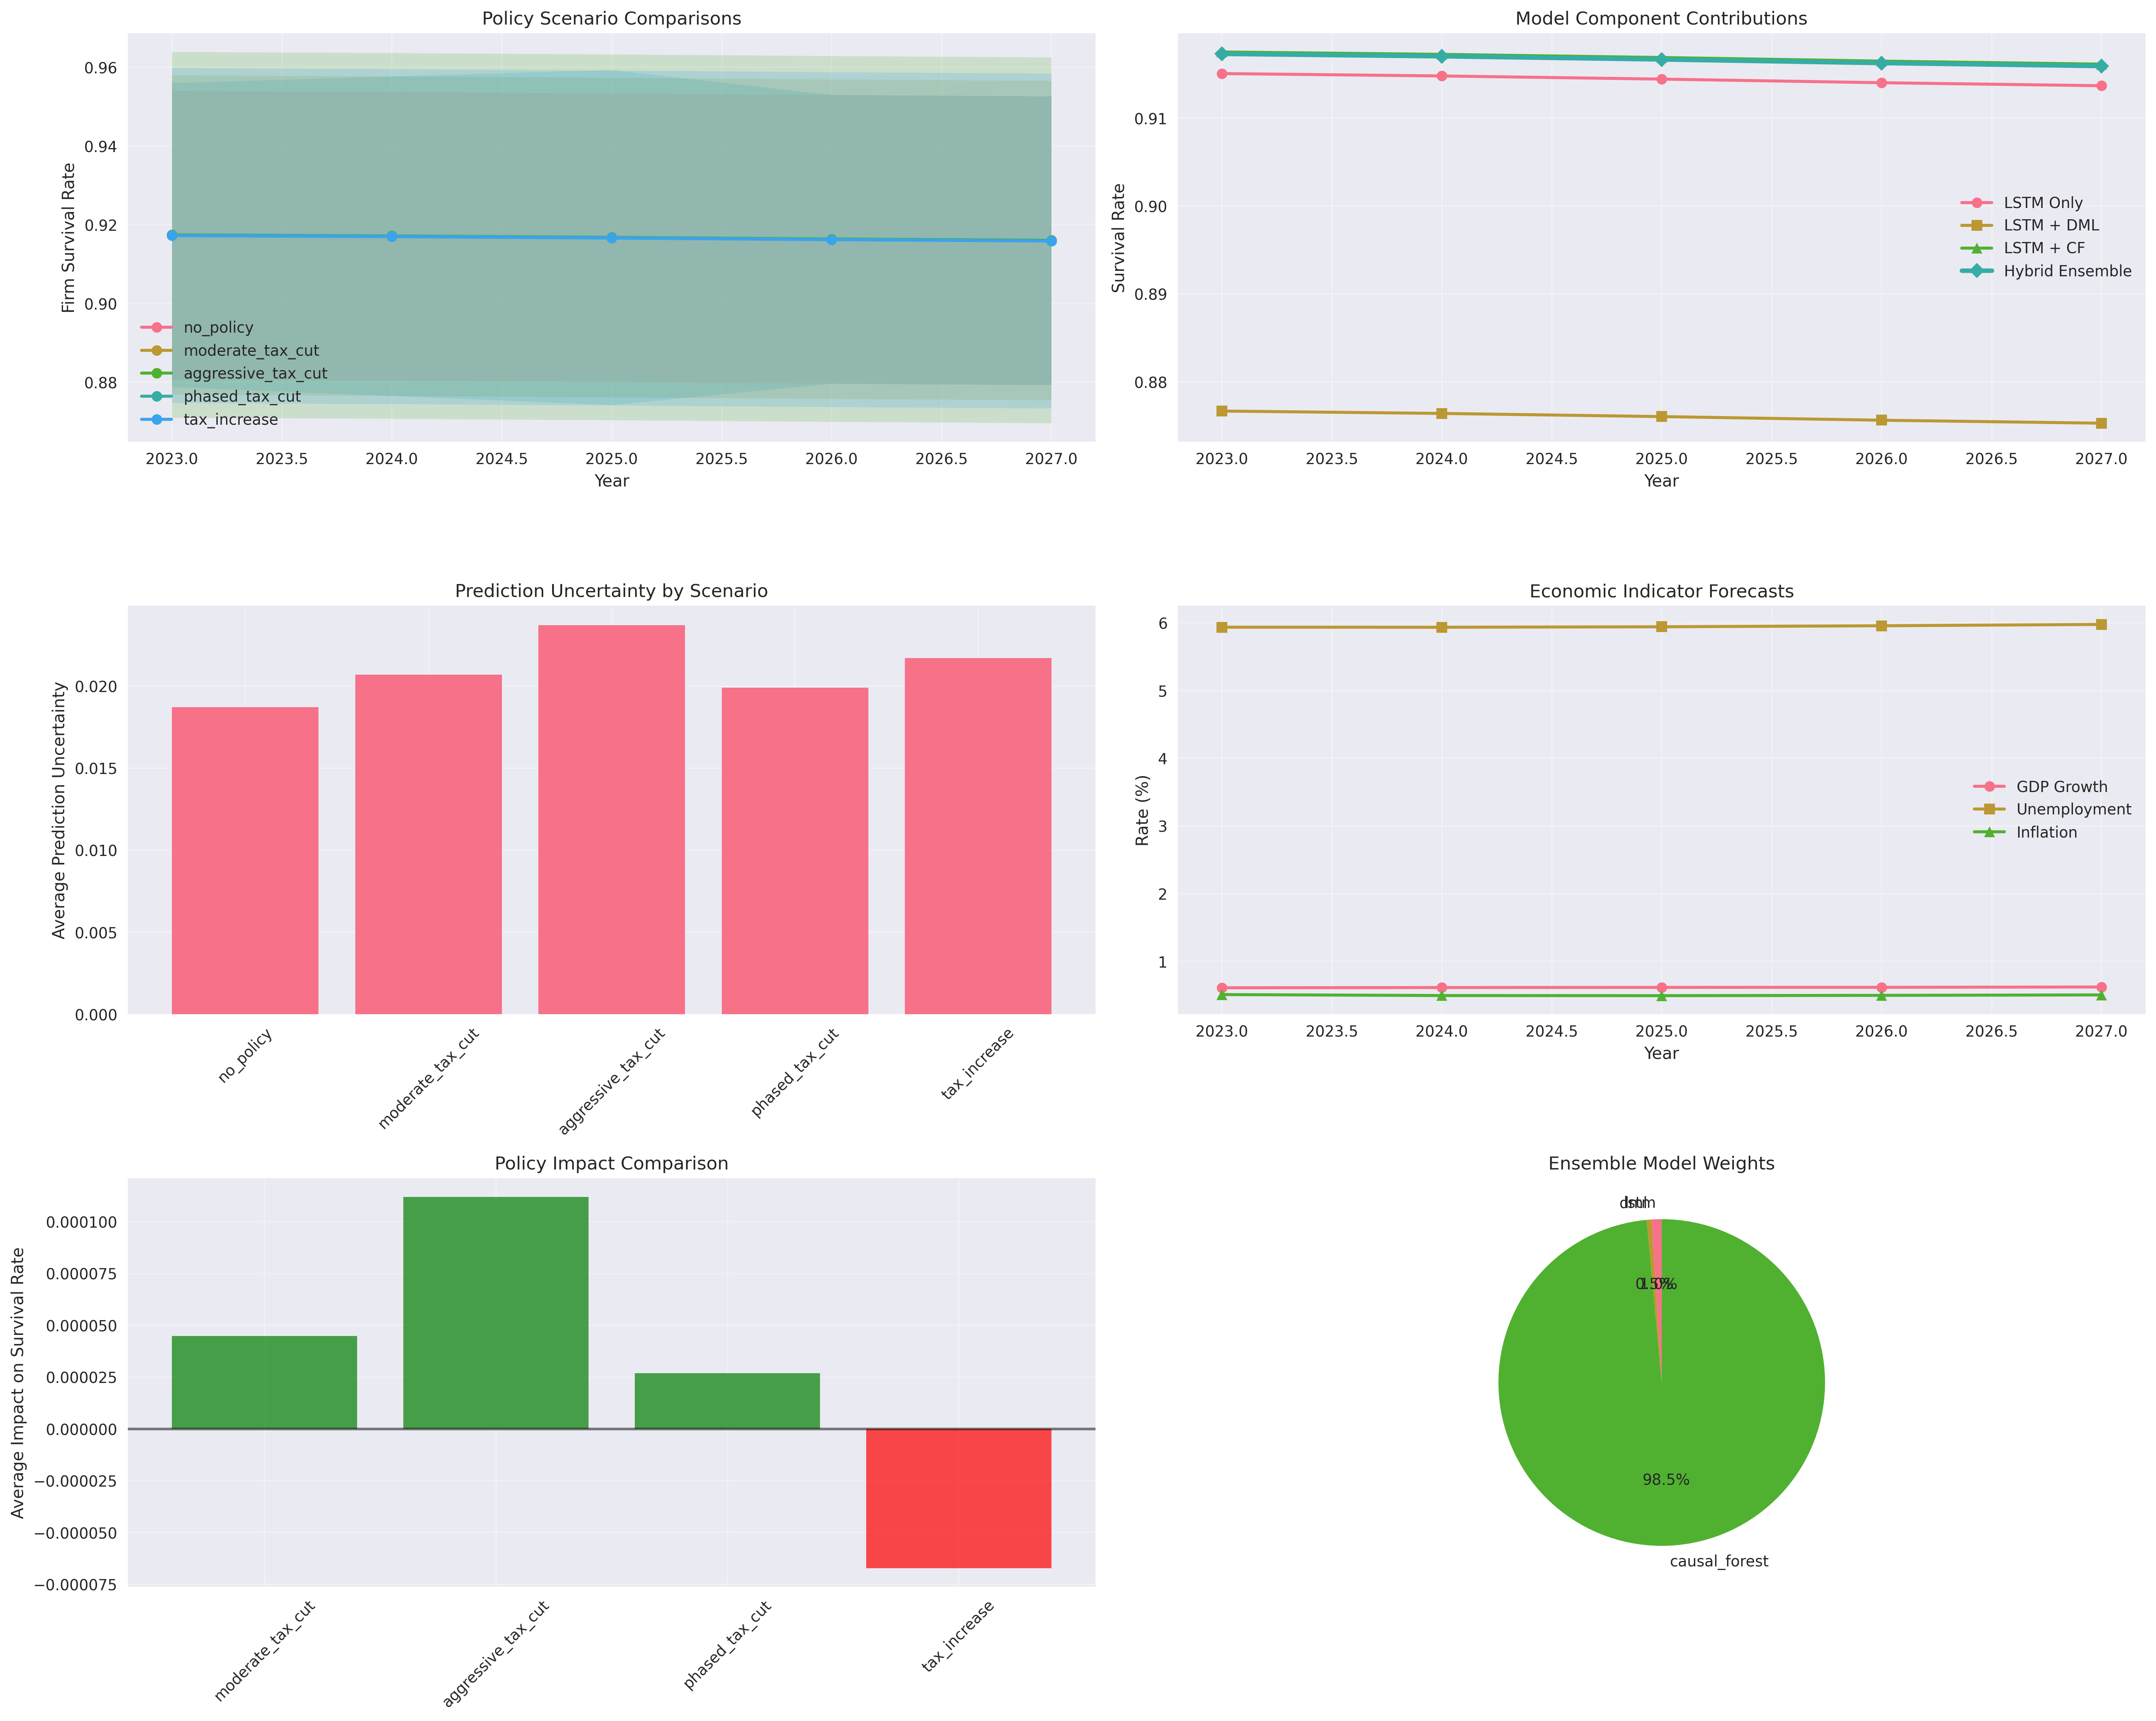
\includegraphics[width=0.85\textwidth]{../figures/hybrid_policy_analysis_comprehensive.png}
  \textit{[Figure placeholder: Macro Indicators and Policy Markers visualization]}
  \caption{Macro Indicators and Policy Markers (Composite Visualization)}\label{fig:econ_overview}
\end{figure}

\subsection{Train/Validation Partitioning}
Temporal splits follow a rolling-origin evaluation design: an initial training window is incrementally expanded while forecasting horizons are evaluated forward. This design mitigates look-ahead bias and aligns with prospective policy simulation use-cases.
